% Este arquivo .tex será incluído no arquivo .tex principal. Não é preciso
% declarar nenhum cabeçalho

\section{Bateria Valorosa}

\begin{figure}[H]
  \centering
  
\includegraphics[scale=0.27]{img/alem_da_graduacao/valorosa_foto1.jpg}
\end{figure}

Criada em 1998 por alunos do IC, a \textbf{Bateria Valorosa} é umas das
baterias mais tradicionais da Unicamp, e você muito provavelmente irá
conhecê-la no primeiro dia de aula.

Ao longo do ano, a Valorosa toca em diversos eventos, como o Intercomp, o
Interbatuc e a UPA, além de se apresentar em festas e apoiar as atletas em
jogos internos da Computação e de outros cursos.

A Valorosa realiza ensaios semanais no IC, para os quais estão todas,
especialmente bixetes e bixos, convidadas a participar. Basta comparecer aos
ensaios, não é necessário saber tocar nenhum instrumento. Quem quiser aprender
é sempre muito bem-vinda na bateria!

Para mais informações sobre a Bateria Valorosa, acesse a página no Facebook.
\begin{compactitemize}
  \item Facebook: \url{fb.com/bateria.valorosa}
\end{compactitemize}

\begin{figure}[H]
  \centering
  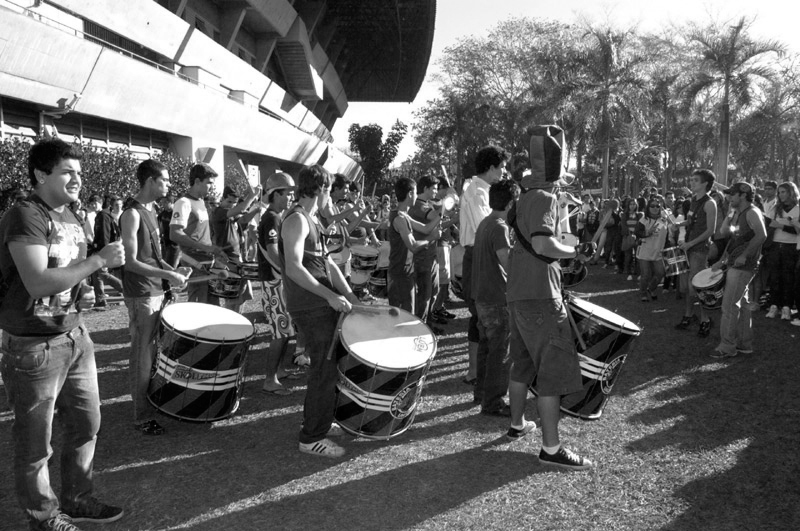
\includegraphics[scale=0.27]{img/alem_da_graduacao/valorosa_foto2.jpg}
\end{figure}
